\documentclass[10pt]{article}

% Venue-neutral anonymous working style. Apply a destination template only after
% the venue, review mode, and page policy are known.
\usepackage[margin=0.85in]{geometry}
\usepackage[numbers,sort&compress]{natbib}

\usepackage[utf8]{inputenc}
\usepackage[T1]{fontenc}
\usepackage{hyperref}
\usepackage{url}
\usepackage{booktabs}
\usepackage{amsmath,amssymb}
\usepackage{microtype}
\usepackage{graphicx}
\usepackage{flafter}
\usepackage{float}
\usepackage{xcolor}
\usepackage{multirow}
\usepackage{siunitx}
\setlength{\emergencystretch}{2em}

\definecolor{frameblue}{HTML}{275DAD}
\definecolor{frameorange}{HTML}{E57A44}
\hypersetup{colorlinks=true,linkcolor=frameblue,citecolor=frameblue,urlcolor=frameblue}
\newcommand{\method}{\textsc{FrameContact}}
\newcommand{\topktwo}{\textsc{TopK2}}
\newcommand{\mpc}{mean-per-complex}
\newcommand{\mpcap}{MPC-AP}

\title{\method: Contact-Derived Task Routing for\\
Antibody--Antigen Interfaces}

\author{Anonymous Authors}
\date{}

\begin{document}

\maketitle

\begin{abstract}
Antibody--antigen interface prediction couples three related outputs: residue-pair
contacts and their antibody-side paratope and antigen-side epitope marginals. A
single jointly trained checkpoint, however, can be suboptimal for one output.
We introduce \method, a partner-conditioned architecture that combines
protein-language-model residue embeddings, sequence-predicted local backbone
frames, an explicit low-rank contact map, and interleaved bidirectional
cross-attention. At inference, antibody and antigen structures are predicted
separately from sequence; no experimental complex coordinates, native complex
pose, or cross-partner geometry are required. Under a
fixed SAbDab2 development protocol, epoch-level diagnostics and a $2\times2$
task ablation show that the fully joint objective gives the strongest epitope
result. The curves are consistent with late overfitting and do not support simple
multitask competition. We therefore retain joint learning
and change only the epitope readout: an epitope expert aggregates the two
strongest predicted contact edges per antigen residue, and deterministic task
routing uses this expert only for epitope while preserving contact and paratope
from the joint baseline. Before full-development retraining, we freeze this route
and evaluate its screen-stage checkpoints once on an antigen-cluster-disjoint
development holdout of 156 complexes. All three seeds improve epitope \mpcap{}
($+0.0057$, $+0.0141$, and $+0.0089$); a paired bootstrap over 49 antigen
clusters gives a cluster-weighted, seed-averaged improvement of $+0.0295$ with
95\% CI $[0.0126,0.0474]$, conditional on the three trained seeds. We then
retrain on the complete 2,565/549 development split using only
sequence-predicted geometry as model input. The routed three-seed validation
medians are 0.0267/0.2438/0.6885 for contact/epitope/paratope MPC-AP. Relative
to matched bound-geometry development checkpoints, the medians change by
$-0.0015/+0.0067/-0.0233$, respectively. This is a development sensitivity
analysis: the 549-complex validation set selects checkpoints, and a
cluster-weighted paired analysis does not establish an epitope improvement.
The fresh156 result validates the earlier routing decision, not the subsequently
retrained checkpoints. These results support task-specific routing while
showing that deployment without experimental structure preserves contact and
aggregate epitope ranking more readily than paratope ranking.
\end{abstract}

\section{Introduction}

An antibody--antigen interface can be represented by a sparse binary matrix
$Y\in\{0,1\}^{L_{\mathrm{Ab}}\times L_{\mathrm{Ag}}}$, where $Y_{ij}=1$ marks a
residue-pair contact. Paratope and epitope labels are deterministic row and
column marginals of the same contact matrix. This relation
makes joint learning attractive, but it also creates a practical model-selection
problem: antigen-residue ranking and preservation of pair-level contacts or
antibody-side residues can favor different checkpoints.

Recent methods have made epitope prediction antibody-aware using bipartite graph
learning, multimodal interaction estimation, or interleaved cross-attention
\citep{liu2024asep,wang2024mipe,ahmed2026epiformer}. We study these design
choices under one frozen SAbDab2 protocol and ask: \emph{does the epitope
gap arise from early optimization, late overfitting, or competition with contact
and paratope supervision?} We then ask whether an epitope-specific readout can
improve antigen-side prediction while retaining the stronger contact and
paratope behavior of the joint model.

Our contributions are:
\begin{itemize}
  \item We formulate contact, paratope, and epitope prediction around one explicit
  residue-pair contact map, combining pretrained sequence features with local
  N/CA/C geometry predicted separately for each partner and interleaved
  bidirectional cross-attention. Experimental complex coordinates are not
  required at inference.
  \item A controlled $2\times2$ task ablation and epoch-level analysis produce
  curves consistent with late overfitting and do not support simple multitask
  competition, motivating us to retain the fully joint objective.
  \item We introduce a single-factor \topktwo{} epitope readout and deterministic
  task routing. The route improves epitope prediction on a previously unused,
  antigen-cluster-disjoint development holdout while leaving contact and
  paratope exactly unchanged.
  \item We bind data, candidate grids, partner panels, checkpoints, and seeds
  with immutable manifests across screening, a cluster-disjoint route
  confirmation, full-development retraining, and a disclosed non-blind
  historical measurement.
  \item On the complete development split, we replace bound-complex model input
  with sequence-predicted partner geometry and quantify the resulting
  task-specific trade-off without accessing the historical or temporal sets.
\end{itemize}

\begin{figure}[t]
  \centering
  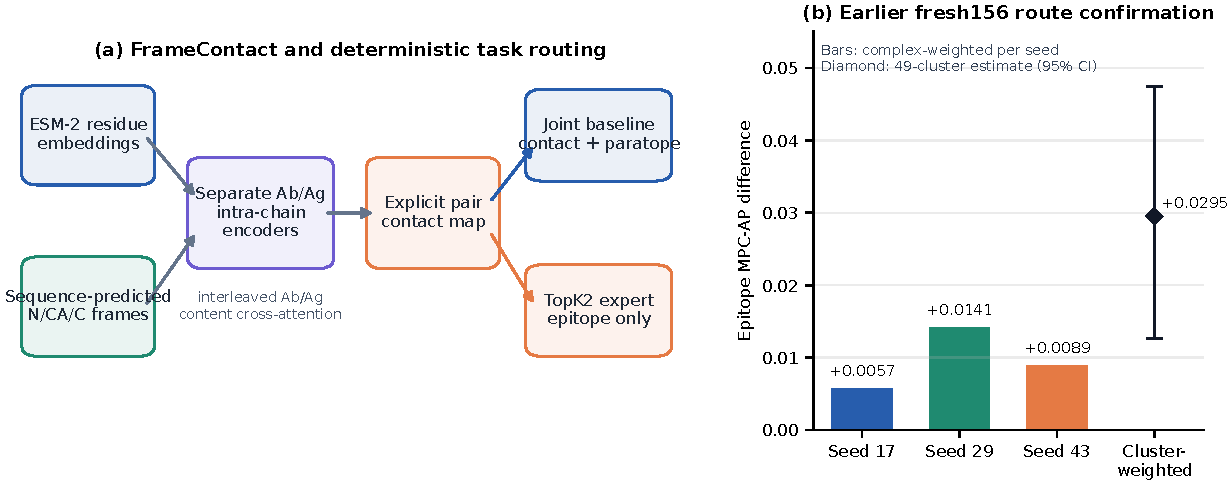
\includegraphics[width=\linewidth]{figures/overview.pdf}
  \caption{\textbf{Model and evidence flow.} \method{} predicts an explicit
  residue-pair contact map from PLM embeddings and sequence-predicted
  intra-chain backbone geometry.
  The joint baseline supplies contact and paratope; the \topktwo{} expert supplies
  epitope only. The route is a fixed task-to-checkpoint map.
  Right: two estimands from the earlier bound-geometry fresh156 route
  confirmation---per-seed complex-weighted gains and the cluster-weighted,
  seed-averaged estimate with its conditional interval.}
  \label{fig:overview}
\end{figure}

\section{Related work}

\paragraph{Antibody-aware interface prediction.}
AsEP provides a clustered benchmark and casts antibody-specific epitope
prediction as bipartite link prediction; its WALLE baseline combines protein
language models with structural graphs \citep{liu2024asep}. MIPE jointly predicts
paratopes and epitopes using multimodal contrastive learning and an estimated
interaction matrix \citep{wang2024mipe}. EpiFormer interleaves bidirectional
cross-attention inside geometric encoders and combines it with sparsity-aware
objectives \citep{ahmed2026epiformer}. SPPIDER-seq demonstrates the value of
partner-conditioned cross-attention in general protein-interface prediction
\citep{porollo2026sppider}. Our EpiFormer-inspired component is a controlled
readout adaptation inside our own 3D pair-contact architecture; the original
EpiFormer and this adaptation have distinct model graphs.

\paragraph{Sequence and structure priors.}
Protein language models such as ESM-2 encode evolutionary regularities into
residue features \citep{lin2023esm}. Geometry-aware graph networks provide useful
inductive biases for molecular coordinates \citep{satorras2021egnn}. Paraplume
shows that PLM representations alone can be strong and scalable for
antigen-agnostic paratope prediction \citep{athenes2025paraplume}. Our setting is
instead partner-specific: antibody and antigen sequences are both inputs, and
their chain-internal geometry is predicted before interface inference. This
removes the need for an experimentally resolved complex at deployment. The
completed experiment still uses experimental structures to derive contact
targets and an auxiliary distance target during training, so we distinguish
sequence-conditioned inference from a fully structure-free training pipeline.

\section{Method}

\subsection{Geometry-aware pair-contact backbone}

For each chain, external ESM-2 embeddings \citep{lin2023esm} are projected to
$d=128$. We construct a right-handed frame $(R_i,o_i)$ at each residue from its
N--C$\alpha$--C atoms, with $o_i$ at C$\alpha$. For an ordered same-chain pair
$(i,j)$, the invariant geometric descriptor is
\begin{equation}
 g_{ij}=\left[\operatorname{RBF}_{16}(\lVert o_j-o_i\rVert),\;
 R_i^\top\operatorname{unit}(o_j-o_i),\;
 \operatorname{vec}(R_i^\top R_j),\;
 \delta_{ij}^{\mathrm{sgn}},\delta_{ij}^{\mathrm{abs}}\right],
 \label{eq:intra-geometry}
\end{equation}
where $\operatorname{unit}(0)=0$ and the two sequence-offset features are
clipped after normalization by 32.
Each antibody or antigen block factorizes intra-chain encoding into (i) dense
content self-attention with sequence rotary positions and (ii) self-attention
whose per-head logits receive an MLP bias from $g_{ij}$. The geometric branch
uses self edges plus at most 32 nearest same-chain neighbors within
\SI{16}{\angstrom}; residues with missing or degenerate frames remain in the
content path but contribute no learned geometric bias. The branches are fused as
$H_{\mathrm{intra}}=H_{\mathrm{dense}}+
\tanh(\gamma_{\mathrm{geo}})(H_{\mathrm{geom}}-H)$, where $H$ is the block
input and $\gamma_{\mathrm{geo}}=0$ at
initialization. Antibody and antigen use separate parameters.

For the deployment-style experiment reported below, backbone coordinates come
from AlphaFold~3 predictions generated separately for the antibody and antigen
components from their sequences, with templates disabled. We retain only each
component's chain-internal N/CA/C geometry: no experimental coordinates,
cross-chain relative coordinates, native complex pose, or true cross-chain
distance is supplied as model input. Experimental bound structures are used to
derive the supervised contact matrix and the auxiliary distance bins during
training, but are not required at inference.

We alternate this intra-chain update with partner exchange rather than applying
one late fusion step. At layer $\ell\in\{1,2\}$, separate geometry-aware encoders
first produce $(A_\ell,G_\ell)$; the shared pair decoder forms a stage contact
map; and bidirectional cross-attention updates both streams before layer
$\ell+1$. Let $h_i^{\mathrm{Ab}}$ and $h_j^{\mathrm{Ag}}$ denote the embeddings
at a given stage. The same directional low-rank decoder is applied in both chain
orders:
\begin{equation}
 \begin{aligned}
 \phi(x,y)&=\frac{q(x)^\top k(y)}{\sqrt{d_p}}+u(x)+v(y)+b,\\
 z_{ij}&=\tfrac12\!\left[
 \phi(h_i^{\mathrm{Ab}},h_j^{\mathrm{Ag}})+
 \phi(h_j^{\mathrm{Ag}},h_i^{\mathrm{Ab}})\right],
 &p_{ij}&=\sigma(z_{ij}),
 \end{aligned}
 \label{eq:contact}
\end{equation}
where $q,k:\mathbb{R}^{d}\rightarrow\mathbb{R}^{d_p}$ are learned projections,
$u,v:\mathbb{R}^{d}\rightarrow\mathbb{R}$ are learned unary maps,
$b\in\mathbb{R}$, and $d_p=128$. The head is evaluated over the complete
antibody--antigen Cartesian candidate grid. Antibody-to-antigen attention at
layer $\ell$ uses
content logits only:
\begin{equation}
 a^{h,\mathrm{Ab}\leftarrow\mathrm{Ag}}_{ij}
 =\operatorname*{softmax}_{j:M_{ij}=1}\!\left(
 \frac{(W_q^h h_i^{\mathrm{Ab}})^\top(W_k^h h_j^{\mathrm{Ag}})}
 {\sqrt{d_h}}\right),
 \label{eq:attention}
\end{equation}
with the analogous update in the reverse direction. Its output is
$A'_{\ell}=A_{\ell}+\tanh(\gamma_{\ell}^{\mathrm{Ab}})
\operatorname{CrossAttn}(A_{\ell},G_{\ell})$, and analogously for $G'_{\ell}$;
both cross-stream gates start at zero. The next intra-chain block consumes these
partner-conditioned features. Thus, local SE(3)-invariant predicted-chain geometry
and partner-specific content exchange are interleaved without supplying the
native cross-chain pose. Although stage contact logits are exposed for
diagnostics, the frozen configuration is
\texttt{content\_only}: no function of $z_{ij}$ enters the attention logits.

Pair supervision is read from the frozen binary contact cohort. Residue labels
are derived strictly from the pair matrix,
\begin{equation}
 y_i^{\mathrm{para}}=\bigvee_j Y_{ij}, \qquad
 y_j^{\mathrm{epi}}=\bigvee_i Y_{ij},
 \end{equation}
rather than imported surface annotations. In the reported joint baseline,
paratope prediction combines a direct antibody-node logit with a masked
log-mean-exp contact marginal, whereas epitope prediction is the logit of the
masked mean pair probability:
\begin{equation}
 \begin{aligned}
 s_i^{\mathrm{para}}
 &=w_p^\top\operatorname{LN}(h_i^{\mathrm{Ab}})
 +\operatorname{LME}_{j:M_{ij}=1}(z_{ij}),\\
 s_j^{\mathrm{epi,base}}
 &=\operatorname{logit}\!\left[
 \operatorname{clip}\!\left(
 \frac{1}{|I_j|}\sum_{i\in I_j}p_{ij},\epsilon,1-\epsilon
 \right)\right],
 \qquad I_j=\{i:M_{ij}=1\},
 \end{aligned}
 \label{eq:baseline-residue-readouts}
\end{equation}
where $\operatorname{LME}_{r\in S}(z_r)=
\log\sum_{r\in S}\exp(z_r)-\log|S|$. Applying a sigmoid gives the residue
probabilities. The joint loss is
\begin{equation}
 \mathcal{L}=\mathcal{L}_{c}+0.1\mathcal{L}_{d}
 +0.1\mathcal{L}_{p}+0.5\mathcal{L}_{e}, \qquad
 \mathcal{L}_{e}=\mathcal{L}_{\mathrm{CB\text{-}BCE}}^{e}
 +\mathcal{L}_{\mathrm{Dice}}^{e}+0.2\mathcal{L}_{\mathrm{prev}}^{e}.
 \label{eq:loss}
\end{equation}
For each complex, binary losses are averaged within each observed class, then
equally across observed classes; complexes also receive equal weight.
$\mathcal{L}_{c}$ uses focal BCE with $\gamma=1$ \citep{lin2017focal}, whereas
$\mathcal{L}_{p}$ and $\mathcal{L}_{\mathrm{CB\text{-}BCE}}^{e}$ use BCE.
With $\varepsilon=10^{-6}$, the epitope-specific terms are
\begin{equation}
 \begin{aligned}
 \mathcal{L}_{\mathrm{Dice}}^{e}
 &=\frac1B\sum_b\!\left[1-
 \frac{2\sum_r p_{br}y_{br}+\varepsilon}
 {\sum_r p_{br}+\sum_r y_{br}+\varepsilon}\right],\\
 \mathcal{L}_{\mathrm{prev}}^{e}
 &=\frac1B\sum_b\left|
 \frac1{n_b}\sum_r p_{br}-\frac1{n_b}\sum_r y_{br}\right|.
 \end{aligned}
 \label{eq:epitope-loss}
\end{equation}
Here, $B$ is the number of complexes in the minibatch, $n_b$ is the number of
valid antigen residues in complex $b$, and $p_{br}$ and $y_{br}$ are the
predicted epitope probability and binary label for residue $r$.
$\mathcal{L}_{\mathrm{Dice}}^{e}$ follows the differentiable Dice objective
\citep{milletari2016vnet}.
$\mathcal{L}_{d}$ is class-balanced cross-entropy on C$\alpha$--C$\alpha$
distances bucketed at $4,8,16,$ and \SI{32}{\angstrom} into five classes; it is
averaged equally over observed classes within each complex and is auxiliary only.

\subsection{Contact-derived epitope expert}

Mean-like marginalization can dilute the few high-confidence edges of a sparse
interface. For antigen residue $j$, the \topktwo{} expert instead computes
\begin{equation}
 \begin{aligned}
 I_j&=\{i:M_{ij}=1\}, & k_j&=\min(2,|I_j|),\\
 \mu_j&=\frac1{k_j}\!\sum_{i\in
 \operatorname{TopK}_{k_j}(\{p_{ij}:i\in I_j\})}p_{ij},
 &s_j^{\mathrm{epi}}&=\operatorname{logit}\!\left(
 \operatorname{clip}(\mu_j,\epsilon,1-\epsilon)\right),
 \end{aligned}
 \label{eq:topk}
\end{equation}
where $\epsilon$ is float32 machine epsilon. Empty candidate sets map to zero
logit, although the complete Cartesian grid prevents this case for real antigen
residues. The only intentionally changed forward computation between the two
training arms is the epitope readout. The backbone, contact decoder,
supervision, loss weights, training data, candidate grid, and
checkpoint-selection rule remain fixed. The \topktwo{} readout participates in
training and supplies the epitope logits used by the epitope loss; it is not a
post-hoc inference-only transformation.

\subsection{Deterministic task routing}

For each seed, we compose the outputs from two independently trained,
seed-matched checkpoints:
\begin{equation}
 \left(\hat P_r^{c},\hat p_r^{\mathrm{para}},\hat p_r^{\mathrm{epi}}\right)=
 \left(f_{\theta_{J,r}}^{c}(x),f_{\theta_{J,r}}^{p}(x),
 f_{\theta_{E,r}}^{e}(x)\right), \qquad r\in\{17,29,43\},
\end{equation}
where $\theta_{J,r}$ is the seed-matched joint baseline checkpoint and
$\theta_{E,r}$ is the seed-matched \topktwo{} expert selected on development
data. The route assigns one frozen checkpoint to each output using fixed task
identity; the routed quantities are continuous scores, not thresholded labels.

\section{Experimental protocol}

\paragraph{Data and splits.}
We use a 3,663-complex SAbDab2 structural cohort \citep{capel2026sabdab2} with a
locally frozen, label-free antigen-fold split; it is not an official SAbDab2
split. Antigen components combine Foldseek reciprocal-min TM-score edges at
$0.5$ with exact PDB-assembly, antigen-sequence, and antibody-sequence identity;
seed 20260730 assigns 2,565/549/549 complexes to train, validation, and the
historical partition with zero exact-identity overlap across roles. Pair labels
come from a frozen binary contact cache over the complete Cartesian candidate
grid (190,509,766 pairs; 143,756 positives). The cache receipt authenticates the
binary labels but does not independently record the upstream atom-level cutoff
or missing-residue policy, so we do not infer either definition from the cache.
For the 3,114 train/validation complexes used in the final sensitivity study,
the antibody and antigen components are predicted separately from sequence and
cached on the same canonical residue axes. Predicted structures for the
historical partition are not materialized. All compared development arms use
the same labels, candidate grid, external embeddings, and 31-way reciprocal
partner panels.

\paragraph{Evidence stages.}
The $512/128$ screen is used for task ablation and route design. Before measuring
fresh156, we freeze the route and remove every instance and antigen cluster used
by earlier selection or confirmation screens, leaving 156 complexes in 49
clusters. This measurement evaluates the frozen screen-stage route. We then
retrain both arms on all 2,565 training complexes and select checkpoints on the
549-complex validation set. We first freeze the route under bound-geometry
development, then repeat the same six seed-and-arm runs after replacing model
input geometry with sequence-predicted partner structures. Consequently,
fresh156 is independent evidence for the preceding routing decision, whereas
the full-development and geometry-replacement tables are validation summaries,
not independent confirmation. The previously exposed 549-complex partition is
reported only as a measurement-only historical appendix result and is not used
in the predicted-geometry study.

\paragraph{Optimization and selection.}
We use three seeds (17, 29, 43), bf16, two interleaved stages, eight heads,
dropout 0.1, AdamW \citep{loshchilov2019adamw} with learning rate
$3\times10^{-4}$ and weight decay $10^{-4}$, and batch size one. Checkpoints
maximize validation epitope \mpcap{}, break ties by contact \mpcap{} and then
earlier epoch, and use at most 20 epochs with
patience 5. The full validation split supplies checkpoint selection, while
fresh156 supplies the earlier antigen-cluster-disjoint route confirmation.

\paragraph{Metrics and statistics.}
We implement ``AUPRC'' as scikit-learn's non-interpolated average precision
(AP; \texttt{average\_precision\_score}), not trapezoidal PR area
\citep{pedregosa2011scikit}:
\begin{equation}
 \operatorname{AP}=\sum_k (R_k-R_{k-1})P_k.
 \label{eq:ap}
\end{equation}
Because positives are sparse and complex sizes vary, the primary metric for task
$t$ averages AP only over positive-eligible complexes
$\mathcal{E}_t=\{n:\sum_\ell y_{n\ell}^{(t)}>0\}$:
\begin{equation}
 \operatorname{MPC\text{-}AP}_t=\frac1{|\mathcal{E}_t|}
 \sum_{n\in\mathcal{E}_t}
 \operatorname{AP}(y_n,s_n),
 \label{eq:mpc}
\end{equation}
with PR metrics preferred to ROC-only summaries under imbalance
\citep{saito2015precision}. Pooled metrics retain all labeled examples, including
those belonging to a zero-positive complex.
Let $\delta_{rn}$ be the routed-minus-joint AP difference for seed $r$ and
complex $n$, and let $C_g$ contain the complexes in antigen cluster $g$. We
report both
\begin{equation}
 \Delta_{\mathrm{seed-med}}=\operatorname*{median}_r
 \frac1N\sum_n\delta_{rn}, \qquad
 \Delta_{\mathrm{cluster}}=\frac1{|G|}\sum_{g\in G}\frac1{|C_g|}
 \sum_{n\in C_g}\frac13\sum_r\delta_{rn}.
 \label{eq:estimands}
\end{equation}
For fresh156, the confidence interval for $\Delta_{\mathrm{cluster}}$ is the
2.5/97.5 percentile interval from 10,000 paired bootstrap resamples of the 49
antigen clusters after first averaging the three fixed seeds. This interval is
conditional on those trained seeds and does not include retraining uncertainty.
The frozen promotion gate required median epitope gain
$\geq0.005$, at least two positive seeds, minimum seed gain $\geq-0.01$, and
exact preservation of routed contact and paratope metrics.

\section{Results}

\subsection{Joint learning remains beneficial}

Both the same-protocol baseline and EpiFormer-inspired model peak early: the
median best epoch across seeds is 2. Training loss continues to fall afterward
while validation epitope AP declines. These curves are consistent with late
overfitting, but do not by themselves identify a unique cause. The controlled task ablation in
Table~\ref{tab:ablation} supports retaining the fully joint objective, which is
strongest; adding contact to epitope-only training is also mildly beneficial.

\begin{table}[H]
\centering
\caption{Three-seed median epitope \mpcap{} on the frozen 512/128
development screen. Architecture, split, and seed set are fixed.}
\label{tab:ablation}
\small
\begin{tabular}{lc}
\toprule
Supervised outputs & Epitope \mpcap{} \\
\midrule
Epitope only & 0.2502 \\
Epitope + paratope & 0.2493 \\
Epitope + contact & 0.2509 \\
Epitope + paratope + contact & \textbf{0.2532} \\
\bottomrule
\end{tabular}
\end{table}

\subsection{Task routing transfers to an unseen development holdout}

On fresh156, the routed model improves epitope \mpcap{} for every seed
(Table~\ref{tab:fresh}). The paired antigen-cluster bootstrap point estimate is
$+0.0295$ with 95\% CI $[0.0126,0.0474]$ for the cluster-weighted,
seed-averaged estimand in Eq.~\eqref{eq:estimands}. Contact and paratope are
exactly unchanged because those outputs are bound to the baseline checkpoint.

\begin{table}[H]
\centering
\caption{Fresh156 epitope \mpcap{} for the screen-stage checkpoints. The route
was frozen before labels from this antigen-cluster-disjoint panel were measured;
these are not evaluations of the later full-development retraining.}
\label{tab:fresh}
\small
\begin{tabular}{lrrr}
\toprule
Seed & Joint baseline & Routed & Difference \\
\midrule
17 & 0.1858 & 0.1915 & +0.0057 \\
29 & 0.1895 & 0.2036 & +0.0141 \\
43 & 0.1849 & 0.1938 & +0.0089 \\
\midrule
Median difference & & & \textbf{+0.0089} \\
\bottomrule
\end{tabular}
\end{table}

\subsection{Sequence-predicted geometry development sensitivity}

We repeat the complete 2,565/549 development protocol after replacing
bound-complex model input with partner-separated AlphaFold~3 predictions. The
model receives no experimental coordinates as input during training or
inference, and no cross-partner geometry is constructed. Table~\ref{tab:full} reports the
three-seed medians on the 549-complex validation set. Because this set also
selects each checkpoint, the comparison is a development sensitivity analysis,
not an independent confirmation.

\begin{table}[H]
\centering
\caption{Full-development validation \mpcap{} with bound-complex versus
sequence-predicted geometry as model input. The final column is the median of
the three seed-matched differences, not the difference between displayed
medians. Validation supplies checkpoint selection for both conditions.}
\label{tab:full}
\small
\begin{tabular}{lrrr}
\toprule
Metric & Bound geometry & Predicted geometry & Paired difference \\
\midrule
Contact & 0.02858 & 0.02673 & $-0.00155$ \\
Epitope & 0.23746 & 0.24378 & $+0.00666$ \\
Paratope & 0.70475 & 0.68847 & $-0.02327$ \\
\bottomrule
\end{tabular}
\end{table}

The predicted-minus-bound epitope differences for seeds 17, 29, and 43 are
$+0.00791$, $+0.00666$, and $-0.01301$; contact differences are $+0.00189$,
$-0.00155$, and $-0.00432$; and paratope differences are $-0.01627$,
$-0.02496$, and $-0.02327$. Thus, the seed-level aggregate keeps contact close
and has a positive median epitope change, but paratope declines consistently.

A complementary paired analysis first averages the three fixed seeds within
each complex and then weights 108 antigen clusters equally. Its
predicted-minus-bound estimates are $-0.00247$ for contact (95\% bootstrap CI
$[-0.00498,0.00003]$), $-0.00563$ for epitope
($[-0.02016,0.00880]$), and $-0.02781$ for paratope
($[-0.03570,-0.02045]$). The apparent epitope direction therefore depends on
the estimand: the median of seed-level aggregate metrics is positive, whereas
the cluster-weighted paired estimate is negative and its interval crosses zero.

\section{Discussion and conclusion}

The curves are consistent with late overfitting, and the task ablation does not
support simple contact/paratope competition as an explanation for the epitope
gap. Contact-derived \topktwo{} aggregation plus deterministic routing produces
a consistent epitope gain on fresh156 under the earlier frozen route. Replacing
experimental model-input geometry with sequence-predicted partner structures
then preserves contact approximately and yields a positive median seed-level
epitope change, but the cluster-weighted epitope interval crosses zero and
paratope declines consistently. This mixed result is stronger evidence for
deployment feasibility than for an overall performance improvement.

Cross-paper numbers from EpiFormer, Paraplume, and other published systems use
different cohorts, splits, labels, and aggregation rules; we therefore do not
treat them as a formal ranking. A defensible structural-method comparison
requires rerunning each baseline on the identical split and candidate grid.
The principal limitations are the absence of an independent evaluation of the
final retrained checkpoints, the paratope sensitivity to predicted geometry,
the use of bound-derived labels and auxiliary distance supervision during
training, and the cache-level provenance boundary on the atom-level contact
definition.

\section*{Reproducibility statement}

Each checkpoint has 2,395,374 parameters. Routing evaluates two checkpoints,
therefore requiring two forward passes. The expert reruns used one RTX 4090 per
seed, bf16, batch size one, and 21.33 aggregate GPU-hours. Frozen ESM-2 input
features use \path{facebook/esm2_t33_650M_UR50D}, revision
\texttt{08e4846e5371}, 1,280 dimensions, and weight SHA-256 prefix
\texttt{a08adabb949f}. The embedding-manifest SHA-256 prefix is
\texttt{9ecbc0881516}.

The bound-geometry reference analyzer SHA-256 prefix is
\texttt{f4368275e38d}. The predicted-geometry campaign and analyzer prefixes are
\texttt{1117a6ac45bd} and \texttt{a4168a919e97}; its model-input structure
manifest prefix is \texttt{bf6ea4a21ff3}. Full digests, split roles, and
binary-contact authorities are stored in the accompanying machine-readable
record.
The accompanying machine-readable metrics file records the compact metrics,
seeds, split roles, and audit status used in this draft. The archive also includes
a machine-readable audit of every bibliographic record.

\bibliographystyle{plainnat}
\bibliography{references}

\appendix
\section{Historical SAbDab2 benchmark}

For transparency, Table~\ref{tab:historical} reports a previously exposed,
single-seed, measurement-only historical benchmark. This partition had already
been accessed, and prior test feedback influenced later development. The present
measurement did not select the route, model, checkpoint, threshold, or
calibration, but it is not a fresh blind test and cannot confirm generalization.
Thresholds were selected on development validation and were not refit here.
Pooled metrics use all 549 complexes; per-complex AP excludes one zero-positive
complex and therefore averages over 548 eligible complexes.

\begin{table}[H]
\centering
\caption{Previously exposed, non-blind, single-seed historical measurement; not
used for model selection. AP columns are non-interpolated average precision.}
\label{tab:historical}
\small
\begin{tabular}{lrrrrr}
\toprule
Task & AUROC & AP & F1 & MCC & MPC-AP \\
\midrule
Contact & 0.9371 & 0.0121 & 0.0370 & 0.0519 & 0.0264 \\
Epitope & 0.6915 & 0.1411 & 0.2119 & 0.1564 & 0.2486 \\
Paratope & 0.9567 & 0.6567 & 0.6440 & 0.6097 & 0.7095 \\
\bottomrule
\end{tabular}
\end{table}

\end{document}
